% ============================================================
% 深圳大学实验报告模板(SZU Experiment Report Template)
% This template can be modified according to the specific requirements of your experiment or project.
% Produced by: Chao Fan and Kewei Ou, AI School of SZU
% ============================================================

\documentclass[a4paper,12pt]{article}

% ----------------------------
% 中文与字体支持
% ----------------------------
\usepackage{fontspec} % 字体支持
\usepackage{xeCJK} % 中文字体支持
\setCJKmainfont{Noto Serif CJK SC} % 设置中文字体(Overleaf自带Noto字体)

% ----------------------------
% 页面设置与常用宏包
% ----------------------------
\usepackage{geometry} % 页面边距控制
\geometry{left=1in, right=1in, top=1in, bottom=1in}

\usepackage{longtable} % 支持长表格
\usepackage{graphicx} % 插入图片
\usepackage{fancyhdr} % 页眉页脚控制
\usepackage{tikz} % 绘制框线等图形
\usetikzlibrary{calc} % 坐标计算
\usepackage{verbatim} % 显示代码块
\usepackage{float} % 控制图片浮动位置([H]参数)
\usepackage{caption} % 更好控制图表标题
\usepackage{subcaption} % 子图支持(如果需要)

% ----------------------------
% 页眉页脚设置
% ----------------------------
\pagestyle{fancy}
\fancyhf{} % 清空默认页眉页脚
\fancyhead[L]{深圳大学实验报告} % 左侧页眉文字
\fancyhead[C]{} % 中间空
\fancyhead[R]{} % 右侧空

% ============================================================
% 文档开始
% ============================================================

\begin{document}

% ============================================================
% 封面页
% ============================================================
\begin{titlepage}
    \centering
    \vspace*{1.5cm}
    \Huge{\textbf{深 \ 圳 \ 大 \ 学 \ 实 \ 验 \ 报 \ 告}}\\[1.2cm]
    
    \Large{课程名称:\underline{\makebox[6cm]{Python程序设计}}}\\[0.6cm]
    \Large{项目名称:\underline{\makebox[7cm]{鸢尾花数据分类与可视化}}}\\[0.6cm]
    \Large{学 \qquad 院:\underline{\makebox[6cm]{人工智能学院}}}\\[0.6cm]
    \Large{专 \qquad 业:\underline{\makebox[10cm]{计算机科学与技术(IEEE荣誉班)}}}\\[0.6cm]
    \Large{指导教师:\underline{\makebox[6cm]{舒婷,樊超}}}\\[0.6cm]
    \Large{报告人:\underline{\makebox[2.5cm]{姜顺元}} \quad 学号:\underline{\makebox[3cm]{2024401029}}}\\[0.6cm]
    \Large{实验时间:\underline{\makebox[6cm]{2025年12月14日}}}\\[0.6cm]
    \Large{提交时间:\underline{\makebox[6cm]{2025年12月14日}}}\\[1.5cm]

    \vfill
    \Large{教务处制}
\end{titlepage}

\newpage

% ============================================================
% 正文部分
% ============================================================

\section{实验目的}

本实验通过Python编程实现对经典Iris(鸢尾花)数据集的探索性数据分析(EDA)和多分类器可视化,主要目标包括:
\begin{itemize}
  \item 掌握使用pandas、seaborn、matplotlib和plotly等库进行数据预处理、统计描述与可视化;
  \item 理解鸢尾花数据集的特征分布与类别可分性;
  \item 实现多种分类器(逻辑回归、线性SVM、决策树)的训练与决策边界可视化;
  \item 掌握交互式2D和3D可视化技术,提升数据分析结果的表达效果。
\end{itemize}

\section{实验概述}

实验以Iris数据集为对象,主要流程如下:
\begin{enumerate}
  \item 数据加载与预处理:使用sklearn加载数据集,划分训练集与测试集;
  \item 探索性数据分析:统计特征分布、绘制箱线图与散点图矩阵,观察各类别间的差异;
  \item 分类器训练:在最具区分度的特征子集上训练多种分类器;
  \item 可视化实现:使用matplotlib/seaborn进行静态分析图,使用plotly生成交互式决策边界、概率热图及3D边界/概率体积渲染,使用HTML展示结果。\textbf{网页可以交互,具有更好的展示效果}。
  \item 基于github进行开发 - https://github.com/qbu-666666/PythonHomeworkProject3
\end{enumerate}

\section{实验实现}

实验分为四个独立Python脚本(task1.py、task2.py、task3.py、task4.py),分别实现不同维度的分类器可视化。所有脚本均使用scikit-learn训练模型、numpy构建网格、plotly生成交互式HTML输出,便于动态观察决策边界与概率分布。

\subsection{task1.py:可视化不同分类器的结果}

该脚本实现三种分类器在petal length与petal width两个特征上的决策边界与概率对比:
\begin{itemize}
  \item 训练Logistic Regression、Linear SVM(启用probability)和Decision Tree(depth=5);
  \item 构建高分辨率2D网格(500×500),预测硬决策区域与后验概率;
  \item 使用make\_subplots创建3行5列布局:每行对应一个分类器,左侧与右侧显示决策区域(彩色填充+黑边真实标签点),中间三列为各物种概率热图(白→该类颜色渐变);
  \item Decision Tree无概率时显示说明文字;
  \item 输出task1.html。
\end{itemize}

\subsection{task2.py:可视化3D Boundary}

该脚本针对二分类(versicolor vs virginica)与三特征(sepal length, petal length, petal width)实现3D决策超平面:
\begin{itemize}
  \item 使用线性SVM训练,计算决策超平面方程;
  \item 构建3D网格,绘制决策平面(Surface)与彩色数据点;
  \item 输出task2.html。
  \begin{figure}[H]
      \centering
      \includegraphics[width=0.6\linewidth]{figs/task2.png}
      \caption{task2.py生成html页面的效果}
      \label{fig:figure1}
    \end{figure}
\end{itemize}

\subsection{task3.py:可视化3D Probability Map}

该脚本在相同二分类与三特征设置下,实现概率分布的3D体积渲染:
\begin{itemize}
  \item 使用RBF核SVM(启用probability)训练;
  \item 构建3D网格,预测概率;
  \item 使用Volume渲染概率体积(透明度表示概率强度),Isosurface绘制P=0.5决策面;
  \item 输出task3.html。
  \begin{figure}[H]
      \centering
      \includegraphics[width=0.4\linewidth]{figs/task3.png}
      \caption{task3.py生成html页面的效果}
      \label{fig:figure2}
    \end{figure}
\end{itemize}

\subsection{task4.py:高级3D多分类可视化}

该脚本扩展到完整三分类,使用Gaussian Process Classifier实现非线性边界:
\begin{itemize}
  \item 构建35×35×35网格,预测平滑概率;
  \item 三子图布局:①每个类P=0.5等值面(Isosurface);②概率体积渲染(Volume,以virginica为例);③交互3D散点图(图例开关类别)。
  \item 输出task4.html。
\end{itemize}

通过以上四个任务,逐步从2D多分类对比深化到3D非线性概率可视化,全面掌握了Python在数据分析与机器学习可视化中的应用。

\section{实验结果}

\begin{itemize}
  \item 探索性分析结果显示:setosa类在所有特征上与其他两类有明显分离;versicolor与virginica在petal特征上高度可分,但在sepal特征上重叠较多。
  \item 2D可视化(task1.html)清晰对比了三种分类器的决策风格:逻辑回归与线性SVM边界平滑且提供可靠概率;决策树边界呈阶梯状,无概率输出。
  \item 3D可视化(task2.html、task3.html、task4.html)揭示了二维投影隐藏的复杂非线性结构,概率等值面与体积渲染直观展示了模型不确定性区域。
\end{itemize}

交互式HTML结果显著优于静态图片,便于动态观察数据分布与模型行为。

\section{讨论与分析}

\begin{itemize}
  \item petal length与petal width是Iris数据集最具区分度的特征组合,适合用于2D决策边界演示;
  \item 不同分类器在该数据集上均取得高准确率,但决策边界形态差异显著:软分类器(逻辑回归、SVM)更适合需要概率输出的场景;决策树边界更易解释但易过拟合;
  \item 交互式可视化(plotly)相比传统matplotlib/seaborn具有明显优势,可hover查看数值、旋转3D视图,大幅提升分析效率与报告表现力;
  \item 3D可视化进一步证明了高维特征空间中非线性模型的优势,同时也暴露了可视化计算开销较大的问题(网格分辨率需权衡);
  \item 本实验证明,python在数据分析和可视化方面有非常大的优势,海量支持库和工具也可以为python语言提供和其他工具(如html)交互的能力,这说明python作为“胶水语言”,易用性和全面性都非常出色。此外,HTML展示效果良好但占用较大,这是该方案的不足之处。
\end{itemize}

\newpage

% ============================================================
% 批阅与成绩评定页
% ============================================================

% 绘制正文外框(包含批阅区域)
\begin{tikzpicture}[remember picture, overlay]
 \draw[thick] 
  ($(current page.north west)+(2cm,-3cm)$) 
  rectangle 
  ($(current page.south east)+(-2cm,2.5cm)$);
\end{tikzpicture}

\vspace{1cm}

% 批阅区
\noindent \textbf{指导教师批阅意见:}
\vspace{5cm}
\hfill

\vspace{1cm}

\noindent \textbf{成绩评定:}
\vspace{2cm}
\hfill

\vspace{1cm}

\noindent \textbf{指导教师签字:}
\vspace{2cm}
\hfill

\vspace{1cm}

% 备注部分
\noindent \textbf{备注:}
\begin{itemize}
 \item 报告内的项目或内容设置,可根据实际情况加以调整和补充。
 \item 教师批改学生实验报告时间应在学生提交实验报告时间后 10 日内。
\end{itemize}

% ============================================================
% 文档结束
% ============================================================

\end{document}